در اینجا سه حالت داریم که از حالت بی‌علامت می‌توانیم با احتمال 
$\frac{1}{3}$
به تمام حالات برویم. از حالت علامت‌دار با احتمال
$\frac{1}{2}$
به خود و حالت مرده می‌توان رفت و در نهایت برای حالت مرده فقط با احتمال یک می‌توان در خود ماند. به این ترتیب برای شکل زنجیره مارکوف آن خواهیم داشت:
\begin{figure}[h]
    \centering
    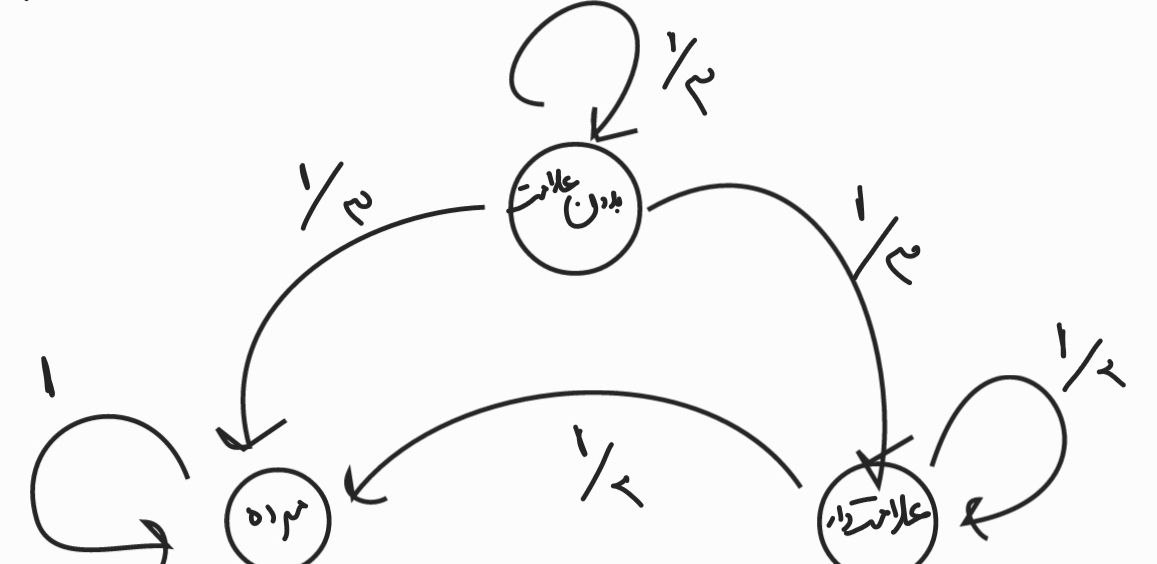
\includegraphics[scale = 0.3]{"commons/second.jpg"}
    \caption{شکل زنجیره مارکوف برای حالت‌های توصیف شده}
\end{figure}

به همین طریق برای ماتریس آن هم خواهیم داشت:
$$\mqty[\frac{1}{3} & \frac{1}{3} & \frac{1}{3} \\ 0 & \frac{1}{2} & \frac{1}{2} \\ 0 & 0 & 1]$$
که در آن سطر و ستون اول مربوط به حالت بدون علامت بوده، سطر و ستون دوم مربوط به بیماران دارای علائم است. همانطور می‌دانیم حالتی جادب است که در نمایش ماتریس آن دارای درایه 
$a_{i, j} = 1$ 
باشد که در اینجا داریم
$a_{3, 3} = 1$
که نشان دهنده جاذب بدن حالت مرده است. حال برای حساب کردن امید ریاضی نیز خواهیم داشت:
$$P_0 = \frac{1}{3}((P_0 + 1) + (P_1 + 1) + 1),\, P_1 = \frac{1}{2}((P_1 + 1) + 1)$$
$$\implies P_1 = 2 \implies 2 P_0 = 5 \implies P_0 = 2.5$$
که نشان‌دهنده این است
$2.5$
روز امید ریاضی زمانی است که طول می‌کشد تا یک فرد سرطاندار بی‌عالمت بمیرد.